\documentclass{article}

\usepackage{amsmath}
\usepackage{amsthm}
\usepackage{amssymb}
\usepackage{bbm}
\usepackage{fancyhdr}
\usepackage{dirtree}
\usepackage{listings}
\usepackage{cite}
\usepackage{graphicx}
\usepackage{enumitem}
\usepackage[margin=1cm]{caption}
\usepackage{subcaption}
\usepackage[pdftex,colorlinks=true, urlcolor = blue]{hyperref}
\usepackage[T1]{fontenc}
\usepackage{inconsolata}
% \lstset{
%     literate={~} {$\sim$}{1}
% }
\usepackage{url}


\newenvironment{claim}[1]{\par\noindent\underline{Claim:}\space#1}{}
\newenvironment{claimproof}[1]{\par\noindent\underline{Proof:}\space#1}{\hfill $\blacksquare$}

\oddsidemargin 0in \evensidemargin 0in
\topmargin -0.5in \headheight 0.25in \headsep 0.25in
\textwidth 6.5in \textheight 9in
\parskip 6pt \parindent 0in \footskip 20pt

% set the header up
\fancyhead{}
\fancyhead[L]{TUM AAS}
\fancyhead[R]{Winter semster 2024}

%%%%%%%%%%%%%%%%%%%%%%%%%%
\renewcommand\headrulewidth{0.4pt}
\setlength\headheight{15pt}
\usepackage{color}
\usepackage{amsmath}
\usepackage{amssymb}
\usepackage{gensymb}
\usepackage{graphicx}
\usepackage{comment,xspace}
\usepackage{hyperref}
%\usepackage{algorithm,algorithmic} 
\usepackage{fancybox}

%\newcommand{\todo}[1]{\par\noindent{\color{red}\raggedright\sc{#1}
%    \par\marginpar{\Large \bf $\star$}}}

%%%%%
%% If you use a font encoding package, please enter it here, i.e.,
%  \usepackage{T1enc}

%% How many levels of section head would you like numbered?
%% 0= no section numbers, 1= section, 2= subsection, 3= subsubsection
%%==>>
\setcounter{secnumdepth}{3}
\graphicspath{{../figs/}}

%%For margin comments
%\newcommand{\todomar}[1]{\marginpar{\tiny\color{red}#1}}
%% Math defs

%For theorems
\newtheorem{assump}{Assumption}
\newtheorem{theorem}{Theorem}[section]
\newtheorem{definition}[theorem]{Definition}
\newtheorem{problem}{Problem}
\newtheorem{lemma}[theorem]{Lemma}
\newtheorem{corollary}[theorem]{Corollary}
\newtheorem{remark}[theorem]{Remark}

\newcommand{\real}{{\mathbb{R}}}
\newcommand{\reals}{\real}
\newcommand{\sphere}{{\mathbb{S}}}
\renewcommand{\natural}{{\mathbb{N}}}
\newcommand{\naturals}{\natural}

\newcommand{\poiss}{\text{Poisson}}
\newcommand{\xfree}{\mathcal X_{\text{free}}}
\newcommand{\xobs}{\mathcal X_{\text{obs}}}
\newcommand{\xgoal}{\mathcal X_{\text{goal}}}
\newcommand{\FMT}{$\text{FMT}^*\, $}


\newcommand{\eps}{\varepsilon}
\newcommand{\He}{H_{\eps}}
\newcommand{\co}{\operatorname{co}}
\newcommand{\ov}{\overline}
\newcommand{\sign}{\operatorname{sign}}
\newcommand{\vers}{\operatorname{vers}}
\newcommand{\union}{\cup}

\newcommand{\map}[3]{#1: #2 \rightarrow #3}
\newcommand{\setdef}[2]{\left\{#1 \; | \; #2\right\}}
\newcommand{\until}[1]{\{1,\dots,#1\}}
\newcommand{\proj}[1]{\operatorname{proj}_{#1}}
\newcommand{\Ve}{\operatorname{Ve}}
\newcommand{\pder}[2]{\frac{\partial #1}{\partial #2}}
\newcommand{\tder}[2]{\frac{d #1}{d #2}}
%\newcommand{\margin}[1]{\marginpar{\tiny\ttfamily#1}}

\newcommand{\subscr}[2]{#1_{\textup{#2}}}

\newcommand{\TSP}{\ensuremath{\operatorname{TSP}}}
\newcommand{\MSP}{\ensuremath{\operatorname{MSP}}}
\newcommand{\MST}{\ensuremath{\operatorname{MST}}}
\newcommand{\OSS}{\ensuremath{\operatorname{OSS}}}
\newcommand{\sRH}{\textup{sRH}\xspace}
\newcommand{\mRH}{\textup{mRH}\xspace}
\newcommand{\mRHFG}{\textup{mRHFG}\xspace}

\newcommand{\card}{\operatorname{card}}

\newcommand{\Vol}{\operatorname{Vol}}
\newcommand{\Area}{\operatorname{Area}}
\newcommand{\limn}{\lim_{n \rightarrow \infty}}
\newcommand{\limni}[1]{\lim_{n_{#1} \rightarrow \infty}}
\newcommand{\diam}{\operatorname{diam}}



%\newcommand{\proof}{\noindent{\bf Proof: \indent}}
%\newcommand{\proofover}{\hfill\vrule height8pt width6pt depth
%                0pt\newline}

\newcommand{\argmin}{\operatornamewithlimits{argmin}}
\newcommand{\reg}{$^{\textrm{\tiny\textregistered}}$}
\newcommand{\liml}{\lim_{\lambda \rightarrow +\infty}}



\newcommand{\p}[1]{\mbox{$\mathbb{P}\left(#1\right)$}} 
\newcommand{\expectation}[1]{\mbox{$\mathbb{E}\left[#1\right]$}} 
\newcommand{\probcond}[2]{\mbox{$\mathbb{P}\left(#1 \,| \, #2\right)$}} 
\newcommand{\condexpectation}[2]{\mbox{$\mathbb{E}\left(#1| #2\right)$}} 
\newcommand{\iteratedexpectation}[2]{\mbox{$\mathbb{E}\left(\mathbb{E}\left(#1| #2\right)\right)$}} 

% Added for KFMT
\newcommand{\LL}{\mathcal{L}}
\newcommand{\M}{\mathcal{M}}
\newcommand{\Mobs}{\mathcal{M}_{\text{obs}}}
\newcommand{\Mfree}{\mathcal{M}_{\text{free}}}
\newcommand{\Mgoal}{\mathcal{M}_{\text{goal}}}
\newcommand{\tx}{\tilde x}
\newcommand{\cl}{\operatorname{cl}}
\newcommand{\VF}{\operatorname{VF}}
\newcommand{\SF}{\texttt{SampleFree}}
\newcommand{\R}{\mathbb{R}}
\newcommand{\N}{\mathbb{N}}
\newcommand{\emin}{\epsilon_{\min}}
\newcommand{\amin}{a_{\min}}
\newcommand{\Amax}{A_{\max}}
\newcommand{\xinit}{x_{\text{init}}}
\newcommand{\pol}{\text{pol}}
\newcommand{\inte}{\text{int}}
\newcommand{\boxw}{\text{Box}^w}
\newcommand{\nti}{n\to\infty}
\newcommand{\ti}{\to\infty}
\newcommand{\X}{\mathcal{X}}
\newcommand{\KFMT}{$\text{KFMT}^*\, $}

\usepackage{outlines}

\usepackage{xparse}
\NewDocumentCommand{\codeword}{v}{%
\texttt{\textcolor{blue}{#1}}%
}
\usepackage{gensymb}

\newcommand{\ssmargin}[2]{{\color{blue}#1}{\marginpar{\color{blue}\raggedright\scriptsize [SS] #2 \par}}}

\newcommand{\Expect}{{\rm I\kern-.3em E}}
 
\usepackage{xcolor}

\setlength{\parindent}{0in}

\title{Autonomous Systems: \\ Group Project: Sub-Terrain Challange}
\author{Bingkun Huang, Haowen Shi, Siyan Li, Weili Tang, Zhenjiang Li}
\date{}

\begin{document}

\maketitle
\pagestyle{fancy}

\section{Introduction}
This project is part of the Sub-Terrain Challenge in the Autonomous Systems course at TUM.
The objective is to develop a system that can autonomously explore a cave environment, detect and locate four objects of interest (lights), and generate a 3D voxel-grid or mesh representation of the environment.
The implementation involves a ROS-based framework, integrating perception, path planning, and control using a quadrotor and a Unity-based simulation.
This document provides an overview of the system architecture, software components, team contributions, challenges, and results, including a ROS graph, figures.

\section{Project Goals}
The project aims to develop an autonomous system capable of exploring a cave environment, detecting and locating four objects of interest (lights) as quickly as possible. Additionally, the system must generate a 3D representation of the environment using either a voxel-grid or a mesh-based approach. Key objectives include:

Implementing a perception pipeline to process depth images and generate point clouds.
Developing path and trajectory planning algorithms for autonomous navigation.
Ensuring seamless ROS integration via a simulation bridge for real-time communication.
Designing a state machine for robot operation, handling take-off, navigation, and landing.


\section{System Overview}

\begin{figure}[h]
    \centering
    \subfloat{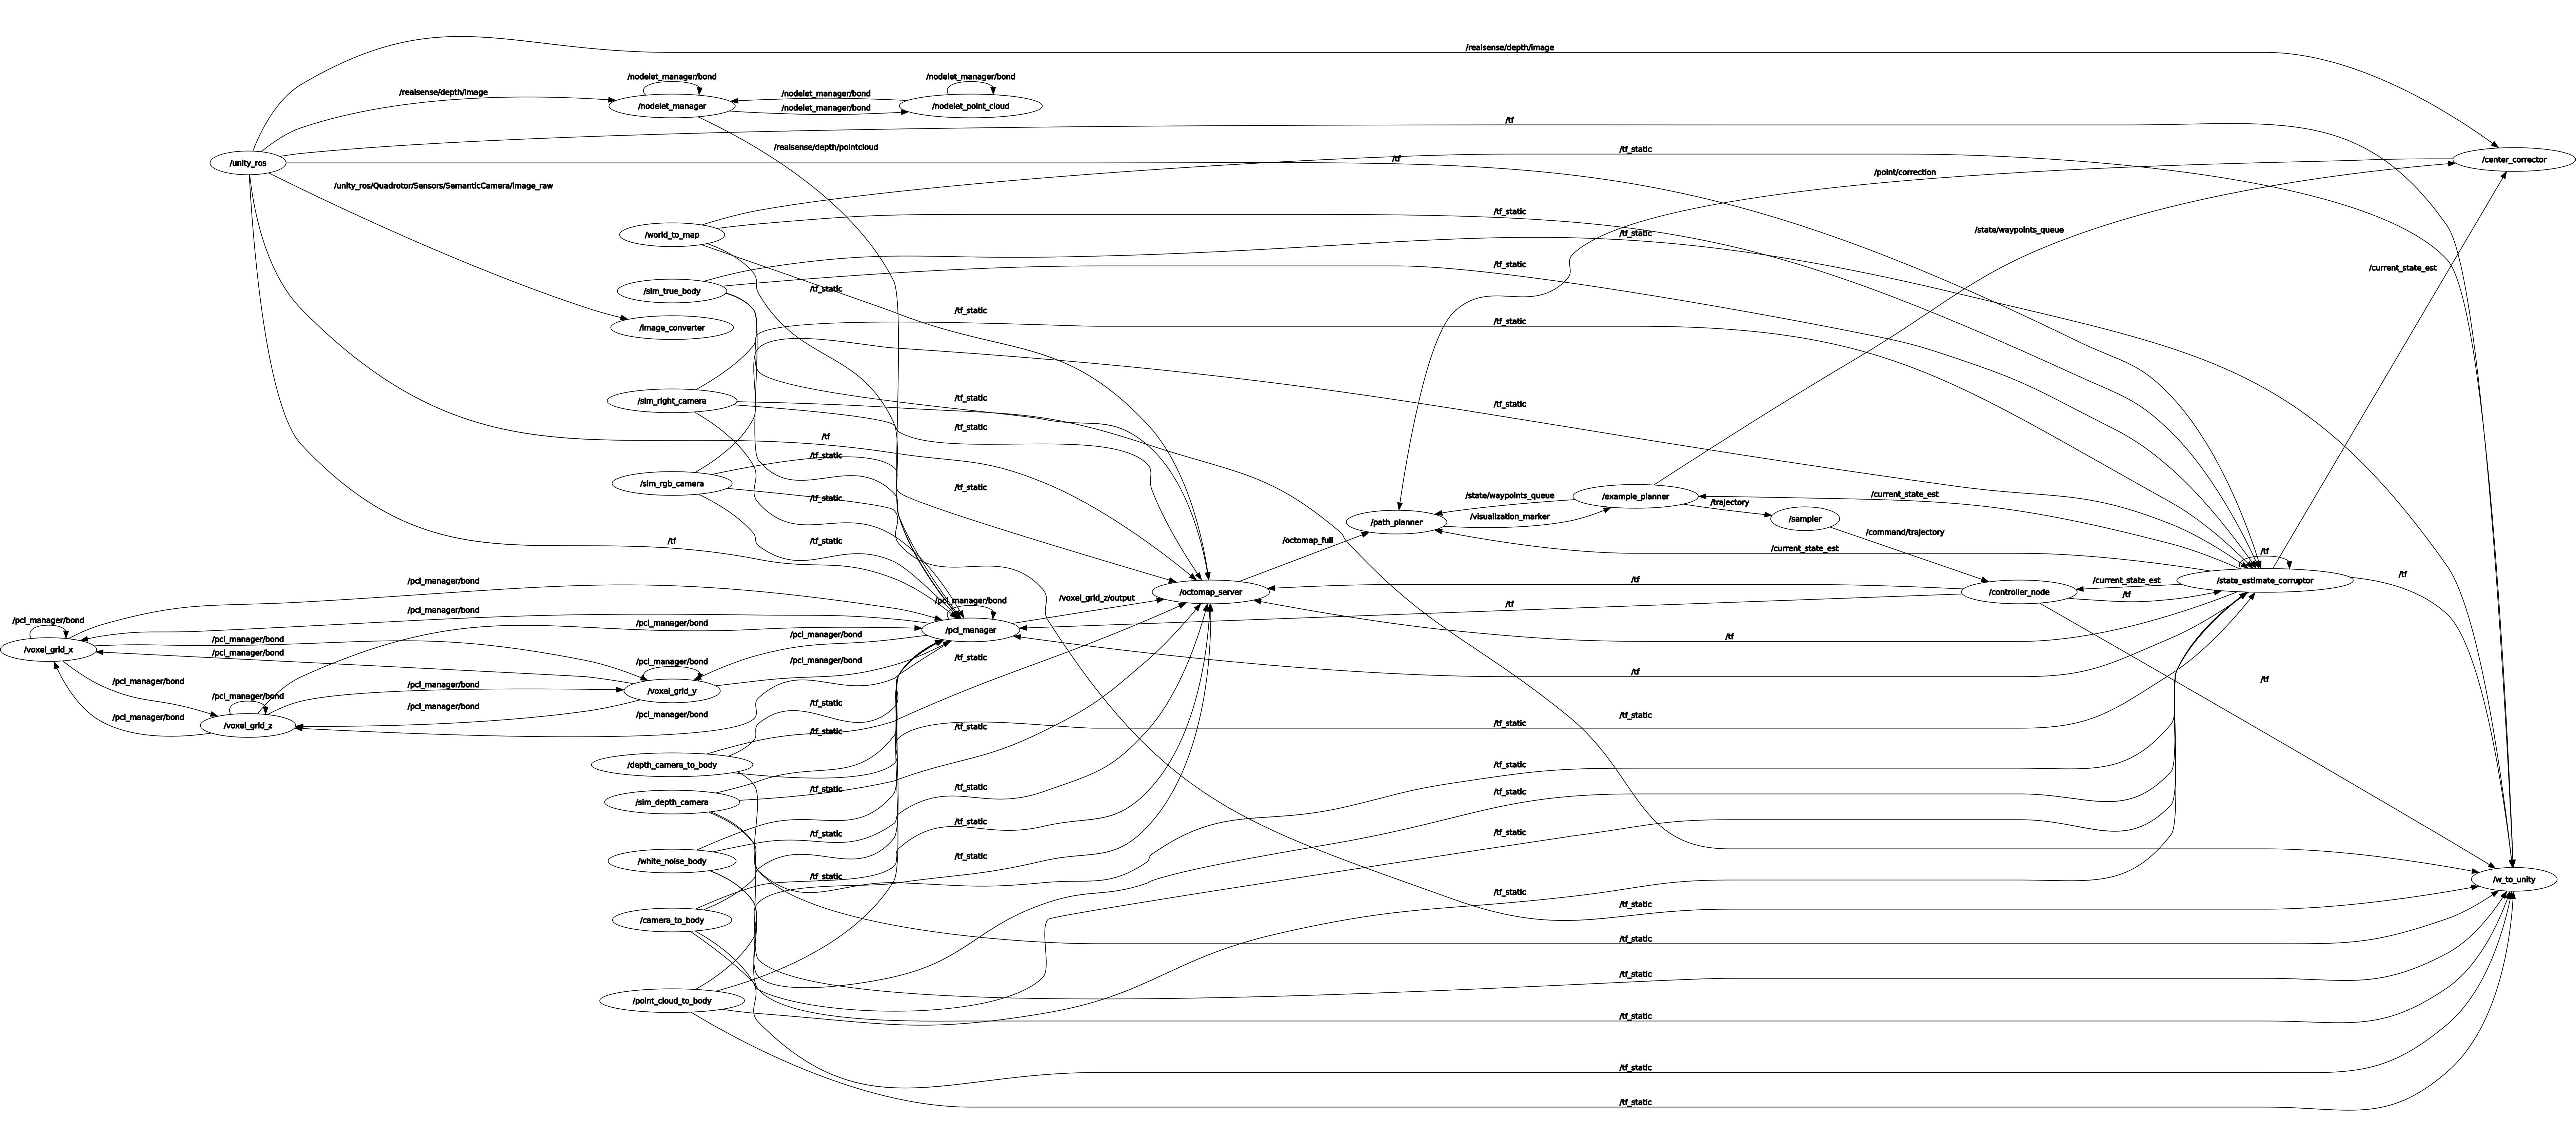
\includegraphics[width=0.8\textwidth]{assets/rosGraph.jpg}}
    \caption{ROS figure of the current project}
    \label{fig:two_images}
\end{figure}



\subsection{Eigen Catkin}
Eigen catkin is a wrapper for the Eigen linear algebra library in ROS (Robot Operating System), ensuring seamless integration within the catkin build system.

In UAV (Unmanned Aerial Vehicle) navigation and control, many critical data structures rely on Eigen, including:
\begin{itemize}
    \item Waypoints: Stored as Eigen::Vector3d (x, y, z) or Eigen::MatrixXd for multiple waypoints.
    \item Current Position: UAV position, velocity, and acceleration are represented using Eigen::Vector3d or Eigen::Affine3d.
    \item Trajectory Optimization: Uses Eigen::MatrixXd for storing trajectory points and performing optimization computations.

\end{itemize}

By providing a standardized Eigen version, eigen catkin prevents dependency conflicts and ensures stable, efficient matrix operations in UAV applications within the ROS ecosystem.

% \subsection{Eigen Check}
% Eigen checks is a ROS-compatible utility library designed to validate and debug Eigen-based numerical computations. It ensures the correctness of matrices and vectors used in robotics applications, particularly in UAVs, autonomous systems, and control algorithms.

% In UAV applications, eigen checks helps verify the correctness of waypoints, positions, velocities, attitudes, and control inputs, reducing errors in navigation and optimization processes.
% By providing robust validation functions, eigen checks improves the reliability of Eigen-based computations in robotics software.


\subsection{Catkin Simple}
Catkin simple is a lightweight CMake wrapper designed to simplify the build process for ROS (Robot Operating System) catkin packages. It reduces boilerplate CMake code, making package management easier and more readable.
Key Features:
\begin{itemize}
    \item Simplifies CMakeLists.txt: Reduces the complexity of manually handling dependencies, libraries, and executables.
    \item Easy Library and Executable Creation: Provides concise functions like cs add library() and cs add executable(), replacing long CMake commands.
    \item Automatic Dependency Management: Automatically links required ROS and system dependencies, reducing manual setup.
    \item Better Build System Integration: Works seamlessly with catkin make, catkin build, and catkin tools.
\end{itemize}

\subsection{ROS Noetic OctoMap}
ROS Noetic OctoMap is the ROS Noetic integration of OctoMap\cite{hornung13auro}, enabling 3D octree-based mapping and environment representation for robot navigation, UAV obstacle avoidance, and path planning. It builds probabilistic 3D occupancy voixel grids from sensor data (i.e. the depth frame image generated by stereo camera system) and lightweight storage with adaptive resolution. In ROS Noetic, octomap server can be used to publish 3D maps. 
\begin{figure}[h]
    \centering
    \subfloat{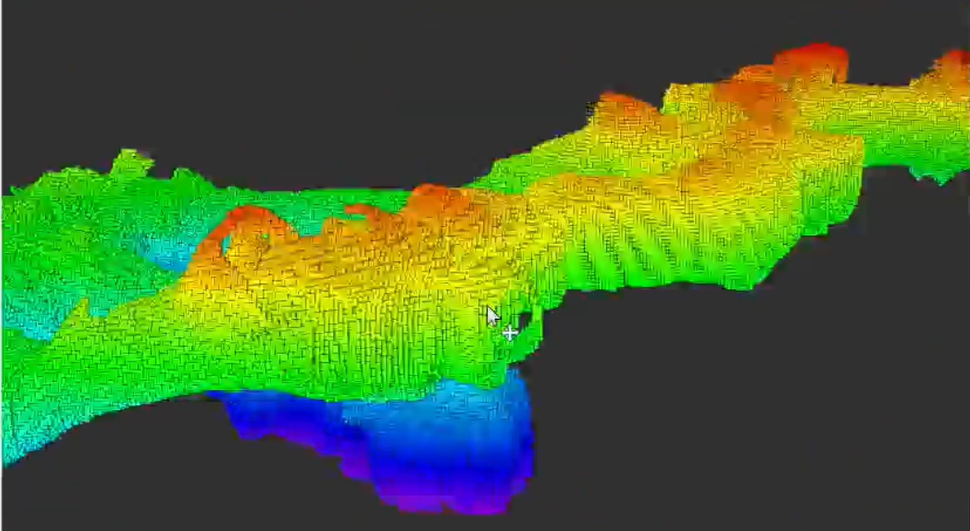
\includegraphics[width=0.8\textwidth]{assets/octomap.jpg}}
    \caption{An example of octomap of the current project map}
    \label{fig:two_images}
\end{figure}

\subsection{Mav Trajectory Generation}
The mav trajectory generation\cite{richter2016polynomial} package provides tools for
polynomial trajectory generation and optimization, specifically designed for micro aerial vehicles, such as quadrotors.
It implements both linear and nonlinear trajectory optimization methods based on minimum snap or minimum jerk approaches, ensuring smooth, dynamically feasible paths for MAV navigation.

The package supports waypoint-based trajectory generation, where users define key positions, and the optimizer calculates continuous polynomial paths. It allows time allocation optimization, ensuring efficient speed profiles. Additionally, it integrates feasibility checks for velocity, acceleration, and thrust constraints to prevent actuator saturation.


\subsection{Flexible Collision Library}
The Flexible Collision Library\cite{6225337} (FCL) is an efficient and versatile collision detection and distance computation library, primarily used in robotics, physics simulation, and computer graphics. It provides a flexible interface supporting rigid body collision detection, nearest point computation, distance queries, and continuous collision detection. FCL utilizes Bounding Volume Hierarchies (BVH) to accelerate collision detection and supports various geometric representations, such as triangle meshes, convex hulls, AABBs, OBBs, and RSS. Widely used in ROS (Robot Operating System) and other robotic simulation frameworks, FCL is capable of handling complex environment modeling and collision detection tasks.

\section{Implementation}

1. Unity Environment

Unity serves as the simulation platform for the entire environment, responsible for simulating realistic physical conditions and providing sensor data to the UAV, including RGB camera and depth camera images. During the simulation, Unity continuously updates the UAV's attitude, position, and camera perspective in real time, ensuring that the sensor data accurately reflects the UAV’s movement within the environment. Additionally, Unity communicates through ROS (Robot Operating System) nodes, allowing external programs to access UAV state information, sensor data, and environmental feedback. This integration enables developers to utilize ROS to subscribe to key sensor data, perform navigation, path planning, and perception tasks, while also sending control commands to Unity for closed-loop control and high-precision simulation. This architecture not only enhances the realism and interactivity of the simulation but also provides an efficient and flexible development environment for research and testing of autonomous UAV systems.
\begin{figure}[h]
    \centering
    \subfloat{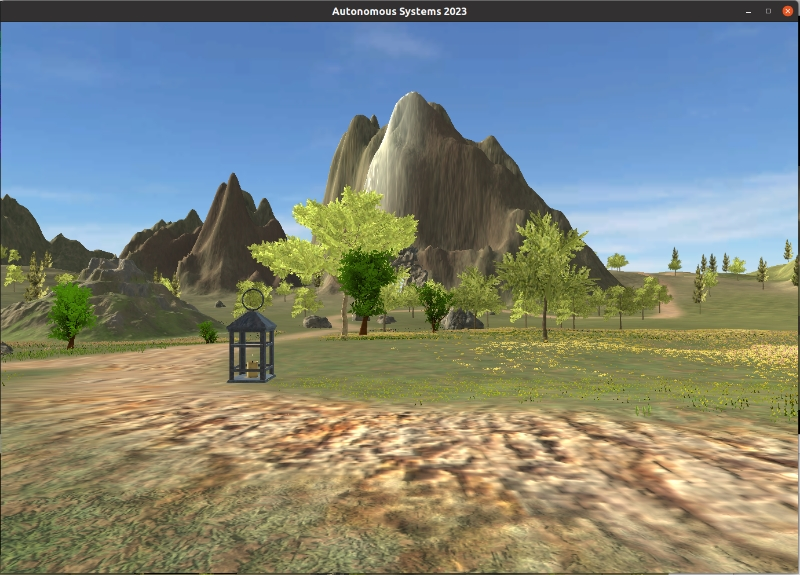
\includegraphics[width=0.8\textwidth]{assets/unity.jpg}}
    \caption{An example of Unity environment of the current project}
    \label{fig:two_images}
\end{figure}

2. Perception

The perception system of the UAV consists of multiple sensors that provide essential data for navigation, mapping, and obstacle avoidance. The system includes an inertial measurement unit (IMU), which measures acceleration and angular velocity to estimate the UAV's attitude and movement. Additionally, the UAV is equipped with two RGB cameras, positioned to capture stereoscopic vision, enabling depth estimation and scene reconstruction. A depth camera further enhances environmental perception by providing precise distance measurements to objects in the surroundings. These sensors work together to enable autonomous decision-making and interaction with the simulated environment in Unity, allowing real-time feedback and control through ROS integration.

Here are some example code used in the project, showing how the information from unity is percepted:
\begin{lstlisting}

    ImageConverter()
    : it_(nh_)
  {
    // Subscrive to input video feed and publish output video feed
    sem_img_sub_ = it_.subscribe(
        "/unity_ros/Quadrotor/Sensors/SemanticCamera/image_raw", 1,
      &ImageConverter::onSemImg, this);

    depth_img_sub_ = it_.subscribe("/realsense/depth/image", 1,
      &ImageConverter::onDepthImg, this);  

    depth_info_sub_ = nh_.subscribe("realsense/depth/camera_info", 1, 
    &ImageConverter::onDepthInfo, this);

    point_pub_ = nh_.advertise<geometry_msgs::PointStamped>(
        "point/latern", 10);

  }
\end{lstlisting}
\begin{figure}[h]
\centering
    \subfloat{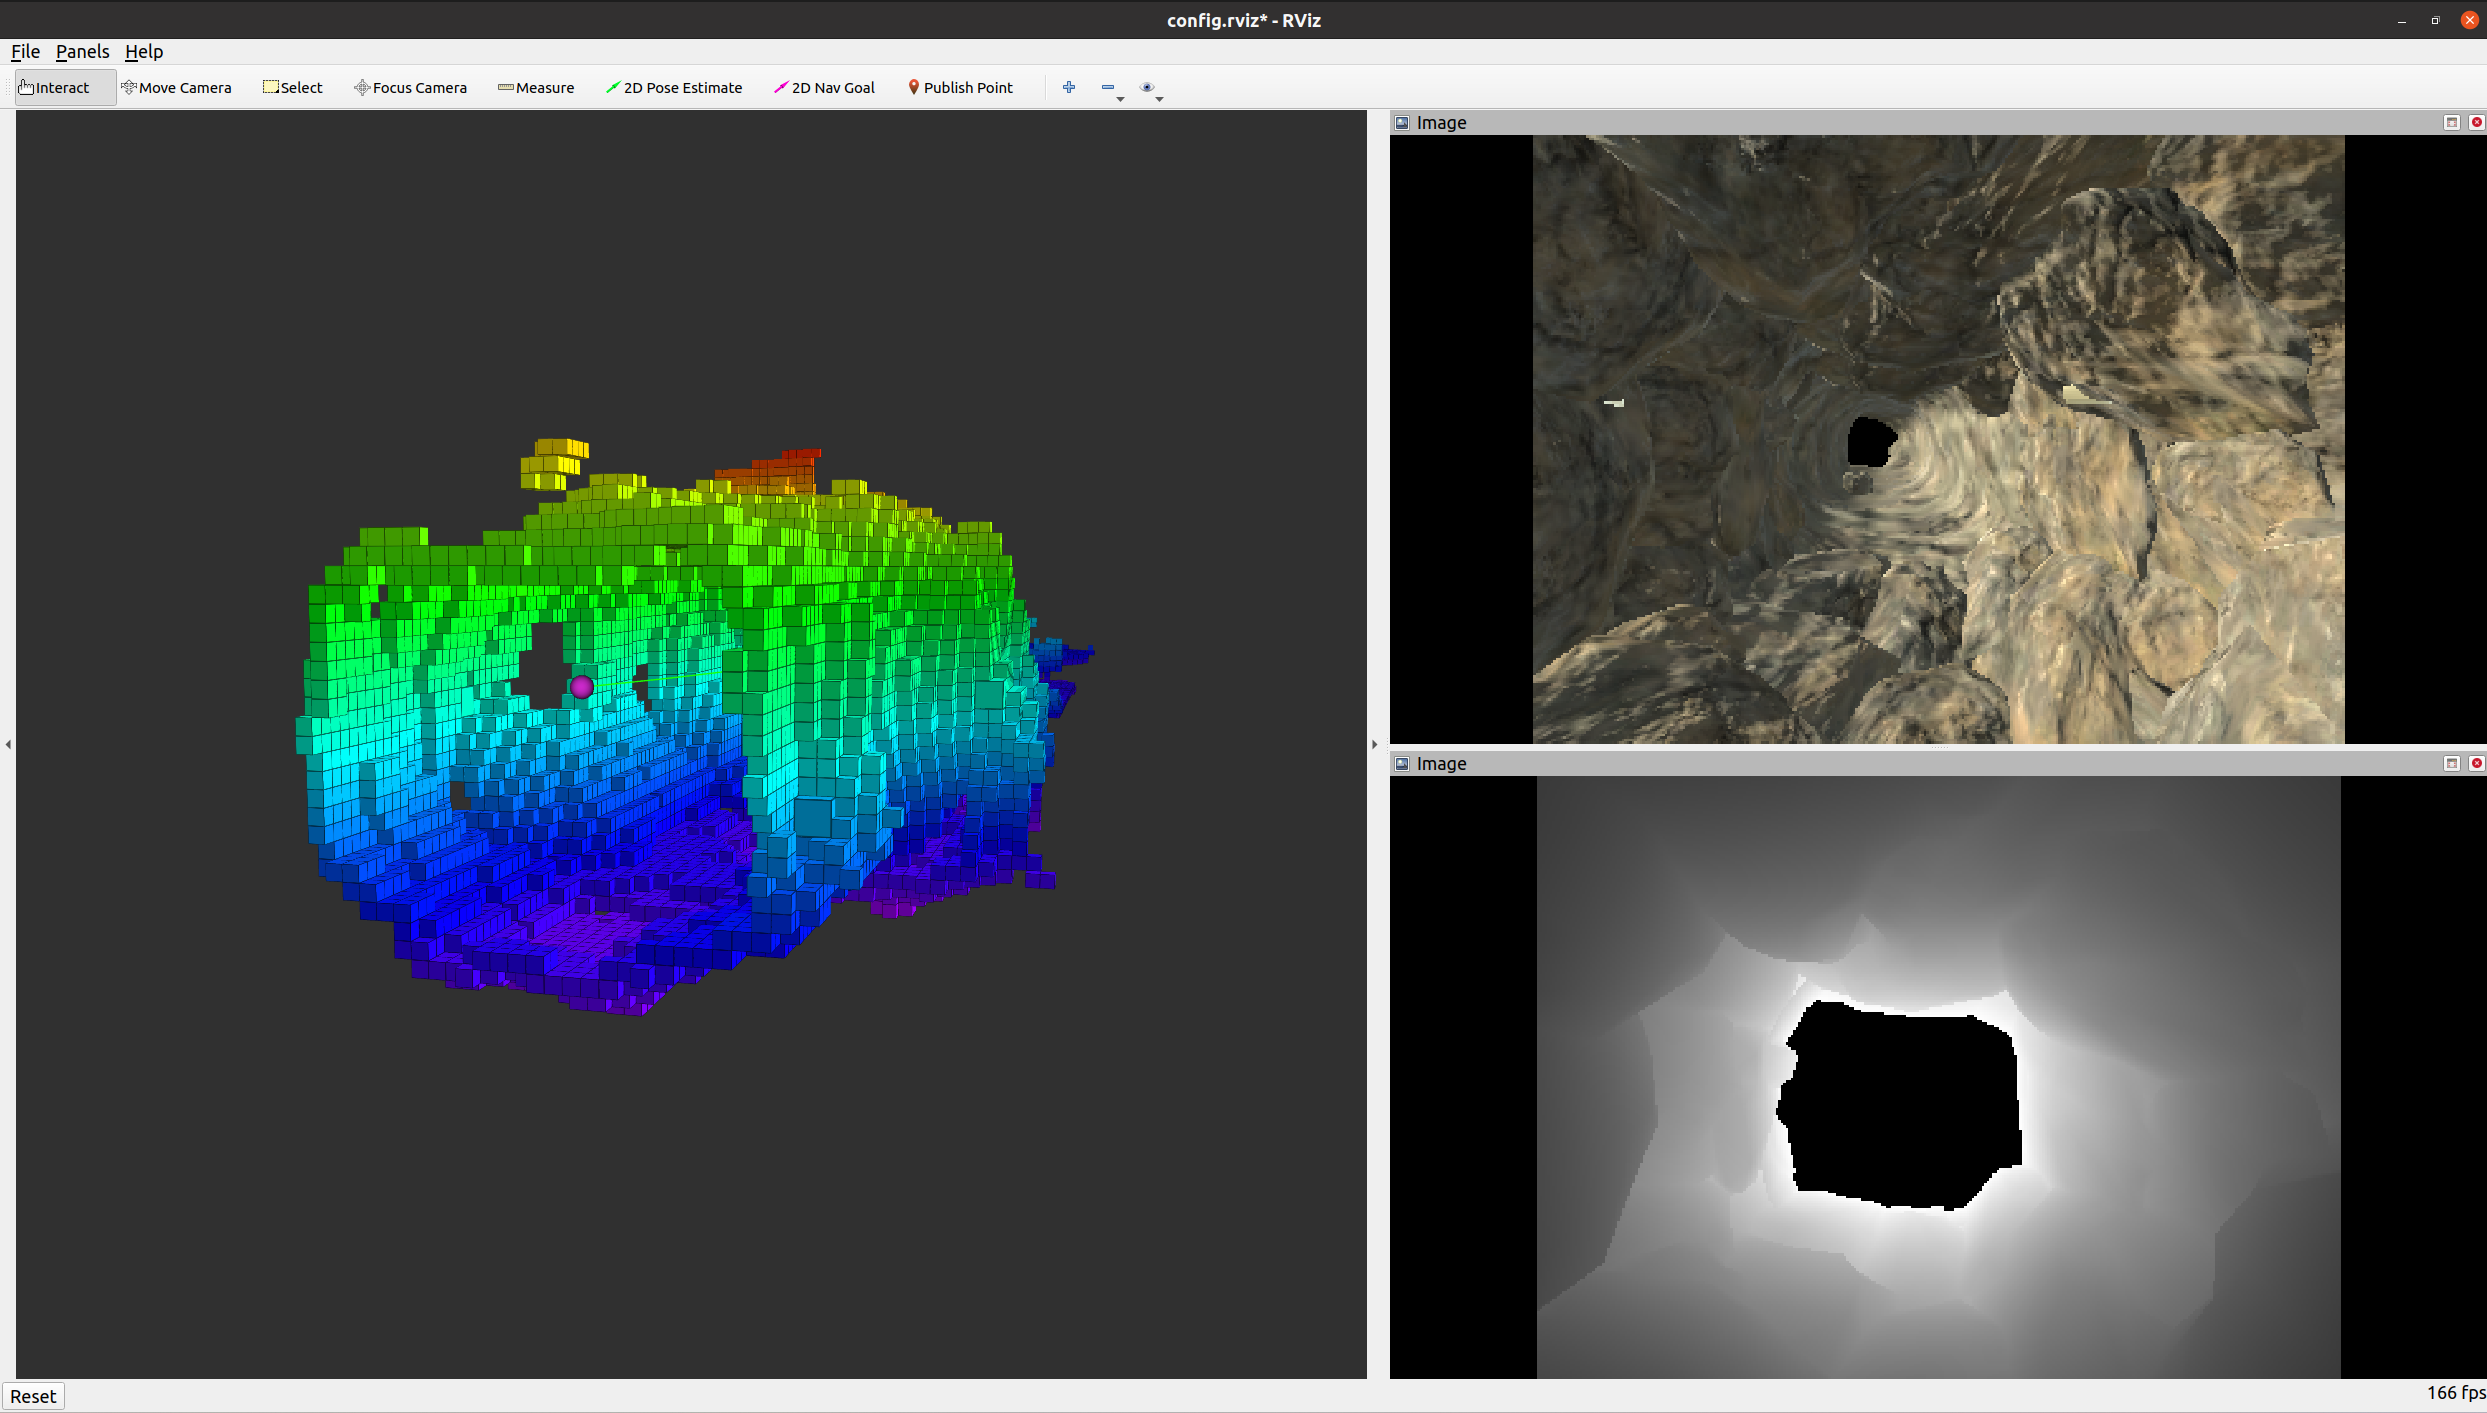
\includegraphics[width=0.8\textwidth]{assets/GUI.jpg}}
    \caption{An example of octomap of the current project map}
    \label{fig:GUI}
\end{figure}

3. From depth image to Octomap

This ROS launch file processes depth data from a RealSense camera to generate a 3D occupancy map (OctoMap). The pipeline begins with two nodelet managers: nodelet\_manager, a general-purpose manager, and pcl\_manager, specifically for Point Cloud Library (PCL) nodelets. The point cloud generation step uses the depth\_image\_proc/point\_cloud\_xyz nodelet to convert a depth image into a 3D point cloud, taking as input:

\begin{lstlisting}{cpp}
    /realsense/depth/image  # Depth image input
    /realsense/depth/camera_info  # Camera info input    
\end{lstlisting}
and producing:

\begin{lstlisting}
    /realsense/depth/pointcloud  # Point cloud output  
\end{lstlisting}

Next, VoxelGrid filtering is applied sequentially along the X, Y, and Z axes to remove NaN values and downsample the cloud to reduce computational load. Each filter is configured with:

\begin{lstlisting}{ymal}
    filter_field_name: X | Y | Z  # Axis to filter
    filter_limit_min: <value>  # Minimum valid range
    filter_limit_max: <value>  # Maximum valid range
    leaf_size: <value>  # Downsampling resolution
\end{lstlisting}

The filtered point cloud is then processed by the octomap\_server node to create the 3D OctoMap, using parameters:
\begin{lstlisting}
    resolution: 1.5  # OctoMap resolution in meters
    frame_id: map  # Reference frame
    sensor_model/max_range: 50  # Maximum sensor range in meters
    \end{lstlisting}

The input to octomap\_server is:
\begin{lstlisting}
    /voxel_grid_z/output  # Filtered point cloud
\end{lstlisting}

4. mini-batch A* specialized for the cave

We uses the A* (A-star) search algorithm\cite{9986703} for path planning and combines it with OctoMap for 3D obstacle avoidance. The whole process can be divided into the following steps:
\begin{itemize}
    \item Subscribe to sensor data
    
    We use ROS to subscribe to OctoMap (3D occupancy map) and target points, which are used for path finding:

    /octomap\_full (from octomap\_server): Gets the 3D map of the current environment for collision detection.
    /point/correction (from FrontierDetecter): Gets the target point from the depth camera to guide the UAV forward.

    \item Preprocess the OctoMap
    
    When receiving OctoMap data, octomapCallback() parses the 3D map and stores it into the octree variable:
    \begin{lstlisting}
    void octomapCallback(const octomap_msgs::Octomap::ConstPtr& msg) {
        std::lock_guard<std::mutex> lock(map_mutex);
        delete octree;
        octree = dynamic_cast<octomap::OcTree*>(
            octomap_msgs::fullMsgToMap(*msg));
        resolution = octree->getResolution();
    }
    \end{lstlisting}

    \item Receive target point
    When a goal point (the location the UAV needs to go to) is received, goalCallback() processes the point:
    \begin{lstlisting}

        void goalCallback(const geometry
        _msgs::PointStamped::ConstPtr& msg) {
            int gx = std::round(msg->point.x / resolution);
            int gy = std::round(msg->point.y / resolution);
            int gz = std::round(msg->point.z / resolution);
            findNearestFree(gx, gy, gz);  

            int sx, sy, sz;
            {
                std::lock_guard<std::mutex> lock(map_mutex);
                octomap::point3d start = 
                octree->keyToCoord(octree->coordToKey(
                    msg->point.x, msg->point.y, msg->point.z));
                sx = std::round(start.x() / resolution);
                sy = std::round(start.y() / resolution);
                sz = std::round(start.z() / resolution);
                findNearestFree(sx, sy, sz);  
            }

            auto path = aStarSearch(sx, sy, sz, gx, gy, gz);
            if (path.empty()) {
                ROS_WARN("A* failed to find a path!");
                return;
            }

            nav_msgs::Path path_msg;
            path_msg.header.frame_id = "map";
            path_msg.poses = path;
            path_pub.publish(path_msg);
            vis_pub.publish(path_msg);
            ROS_INFO("Path published with %ld points.", path.size());
        }
\end{lstlisting}

    \item A* search
    The A* algorithm is implemented in aStarSearch(), which is used to find the optimal path from the starting point to the goal point:

    \begin{lstlisting}

        std::vector<geometry_msgs::PoseStamped> aStarSearch(
            int sx, int sy, int sz, int gx, int gy, int gz) {
        std::priority_queue<Node*, std::vector<Node*>,
         CompareNode> openList;
        std::unordered_map<std::string, Node*> allNodes;

        Node* startNode = new Node(sx, sy, sz);
        Node* goalNode = new Node(gx, gy, gz);
        openList.push(startNode);
        allNodes[hashKey(sx, sy, sz)] = startNode;

        while (!openList.empty()) {
            Node* current = openList.top();
            openList.pop();

            if (current->isGoal(goalNode))
             return reconstructPath(current);

            for (auto& shift : shifts) {
                int nx = current->x + shift[0];
                int ny = current->y + shift[1];
                int nz = current->z + shift[2];

                if (isCollision(nx, ny, nz)) continue;

                Node* neighbor = new Node(nx, ny, nz, current);
                neighbor->g = current->g + 1;
                neighbor->h = std::sqrt(pow(nx - gx, 2)
                 + pow(ny - gy, 2) + pow(nz - gz, 2));

                std::string key = hashKey(nx, ny, nz);
                if (allNodes.find(key) == allNodes.end()
                 || neighbor->g < allNodes[key]->g) {
                    allNodes[key] = neighbor;
                    openList.push(neighbor);
                }
            }
        }
    return {};
}

    \end{lstlisting}

    \item Calculate the path and publish
    When A* finds a path, it calls reconstructPath() to convert the path to the ROS-compatible nav\_msgs::Path format:

    \begin{lstlisting}
        std::vector<geometry_msgs::PoseStamped>
            reconstructPath(Node* node) {
            std::vector<geometry_msgs::PoseStamped> path;
            while (node) {
                geometry_msgs::PoseStamped pose;
                pose.pose.position.x = node->x * resolution;
                pose.pose.position.y = node->y * resolution;
                pose.pose.position.z = node->z * resolution;
                path.push_back(pose);
                node = node->parent;
            }
            std::reverse(path.begin(), path.end());
            return path;
        }

    \end{lstlisting}
    
\end{itemize}

5. Trajectory Generation

The TrajectoryPublisher class initializes with default values for linear and angular scales, setting the trajectory duration to 5 seconds. It sets up publishers and subscribers for the desired state, keyboard input, and current pose. The main loop runs at 50Hz, and if the system is initialized (is\_initialized\_ == true), it generates a trajectory, publishes the desired state, and broadcasts the TF transform. The keyboard input callback updates goal\_pose\_ based on user input and resets the trajectory start time:
\begin{lstlisting}
    void keyboardCallback(const geometry_msgs::Pose& msg) {
        goal_pose_ = msg;
        trajectory_start_time_ = ros::Time::now();
    }
\end{lstlisting}

The current pose callback initializes desired\_pose\_ and goal\_pose\_ with the current pose if the system is not initialized and continuously updates current\_pose\_ from odometry data:
\begin{lstlisting}
    void currentPoseCallback(const nav_msgs::Odometry::ConstPtr& msg) {
    if (!is_initialized_) {
        desired_pose_ = msg->pose.pose;
        goal_pose_ = msg->pose.pose;
        is_initialized_ = true;
    }
    current_pose_ = msg->pose.pose;
}

\end{lstlisting}
The trajectory generation function computes a smooth 3rd-order polynomial trajectory from current\_pose\_ to goal\_pose\_, determining the intermediate desired state (desired\_pose\_) based on elapsed time:

\begin{lstlisting}
    void generateTrajectory() {
    double t = (ros::Time::now() - trajectory_start_time_).toSec();
    if (t > trajectory_duration_) {
        desired_pose_ = goal_pose_;
    } else {
        double alpha = t / trajectory_duration_;
        desired_pose_.position.x = (1 - alpha)
         * current_pose_.position.x + alpha * goal_pose_.position.x;
        desired_pose_.position.y = (1 - alpha)
         * current_pose_.position.y + alpha * goal_pose_.position.y;
        desired_pose_.position.z = (1 - alpha)
         * current_pose_.position.z + alpha * goal_pose_.position.z;
    }
}

\end{lstlisting}
The desired state is then published as a MultiDOFJointTrajectory message:

\begin{lstlisting}
    void publishDesiredState() {
        trajectory_msgs::MultiDOFJointTrajectory msg;
        msg.points.resize(1);
        msg.points[0].transforms[0].translation.x = desired_pose_.position.x;
        msg.points[0].transforms[0].translation.y = desired_pose_.position.y;
        msg.points[0].transforms[0].translation.z = desired_pose_.position.z;
        desired_state_pub_.publish(msg);
    }    
\end{lstlisting}
Finally, the broadcast transform function publishes desired\_pose\_ as a TF transform with the frame ID "av-desired":

\begin{lstlisting}
    void broadcastTransform() {
    static tf::TransformBroadcaster br;
    tf::Transform transform;
    transform.setOrigin(tf::Vector3(desired_pose_.position.x,
     desired_pose_.position.y,
     desired_pose_.position.z));
    transform.setRotation(tf::Quaternion(desired_pose_.orientation.x,
     desired_pose_.orientation.y, desired_pose_.orientation.z,
      desired_pose_.orientation.w));
    br.sendTransform(tf::StampedTransform(transform, ros::Time::now(),
     "world", "av-desired"));
}
 
\end{lstlisting}


\section{Results}

\begin{figure}[h]
    \centering
        \subfloat{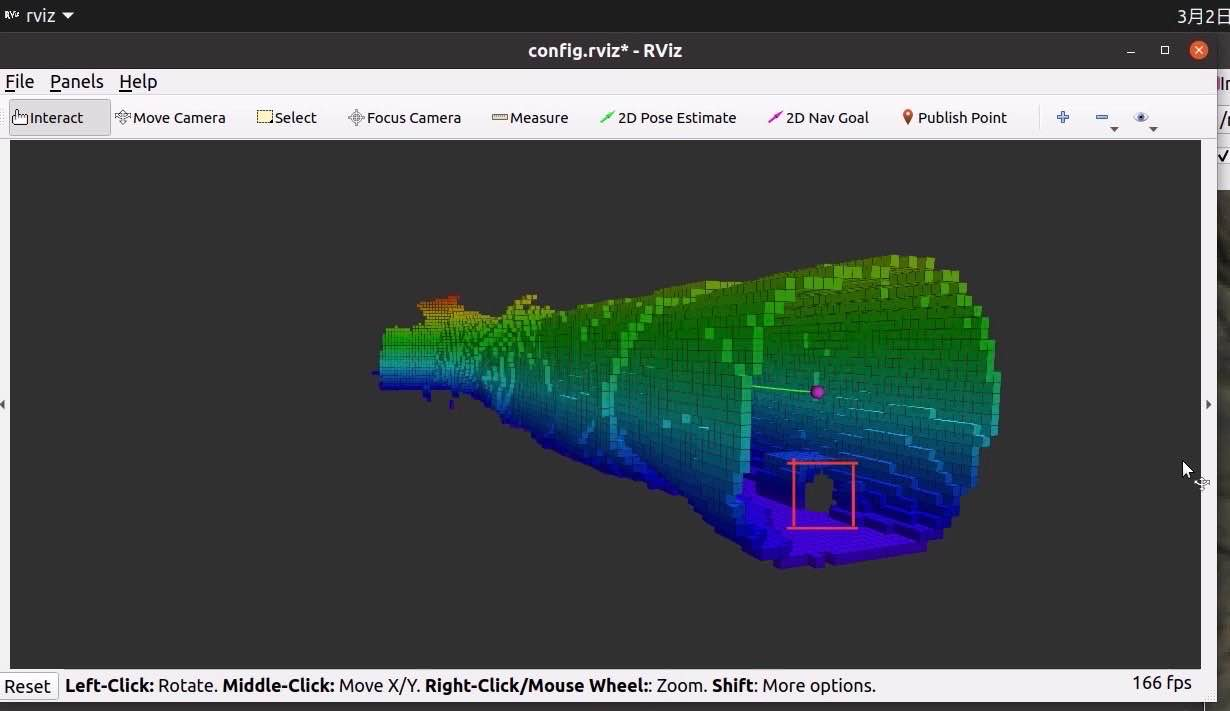
\includegraphics[width=0.5\textwidth]{assets/mark}}
        \caption{An example of target rendered in octomap while the UAV is flying}
        \label{fig:GUI}
    \end{figure}

    \begin{figure}[h]
        \centering
            \subfloat{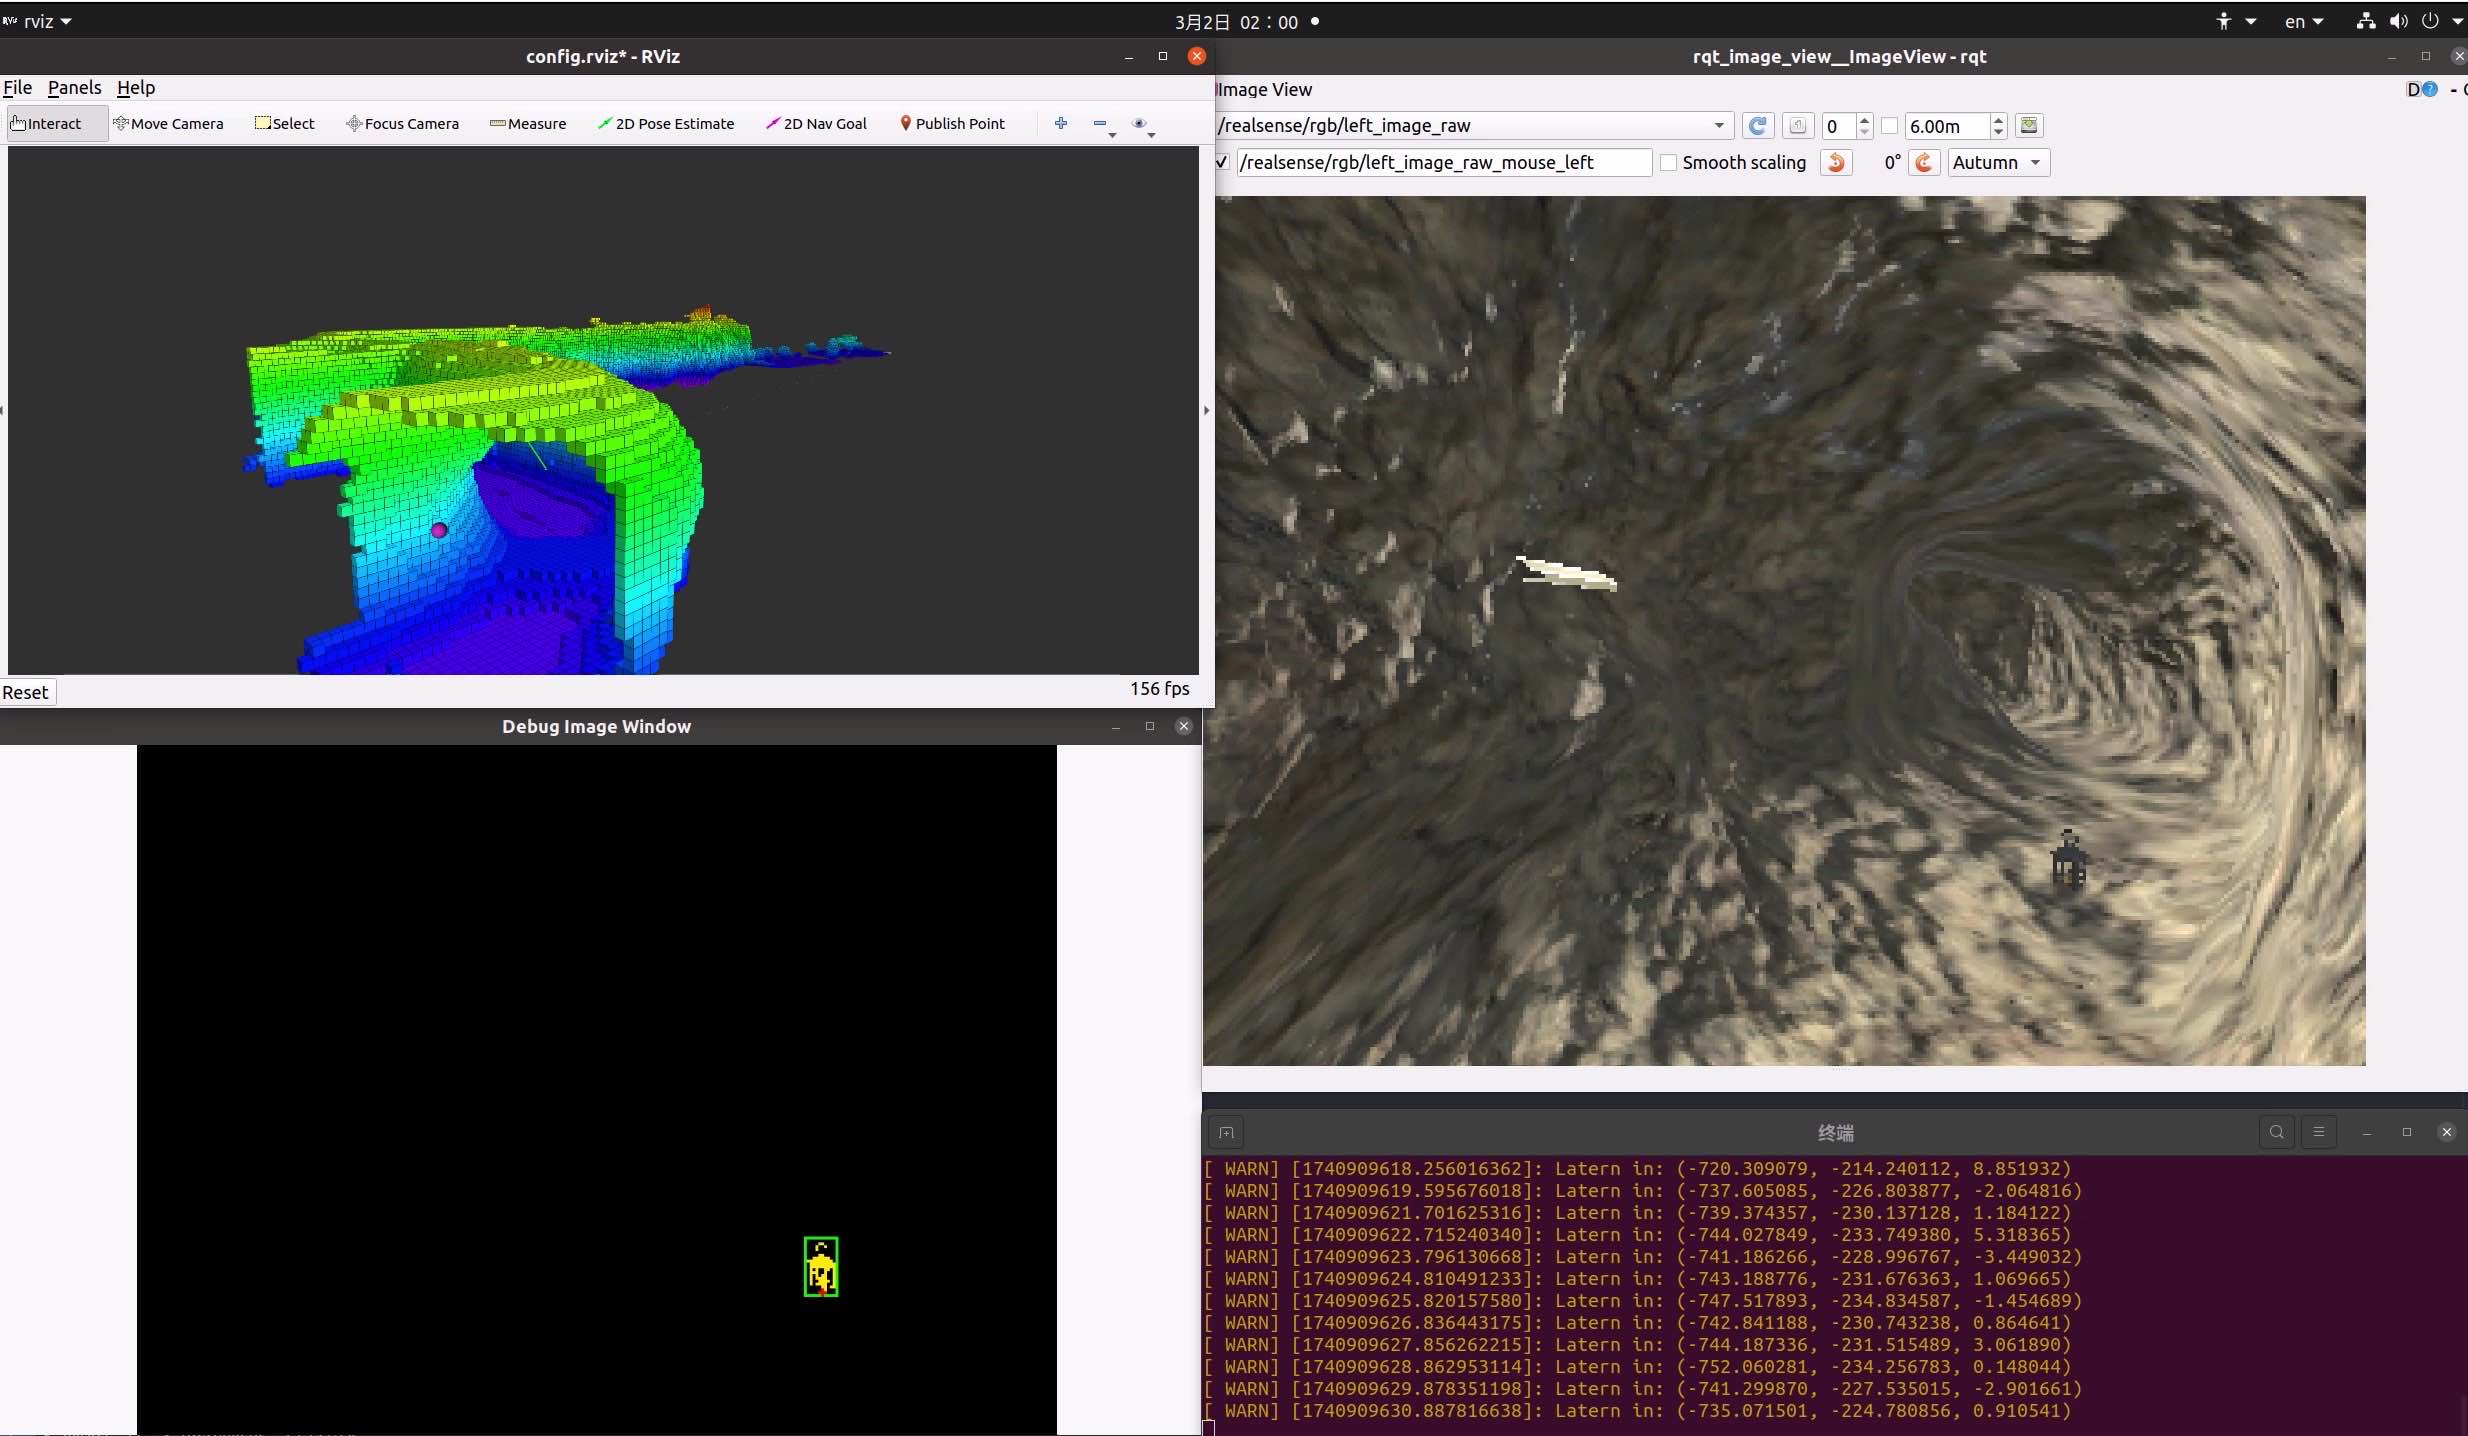
\includegraphics[width=0.5\textwidth]{assets/semantic}}
            \caption{An example of target detected and showed in semantic camera, while the UAV is flying}
            \label{fig:GUI}
    \end{figure}

    \begin{figure}[h]
        \centering
            \subfloat{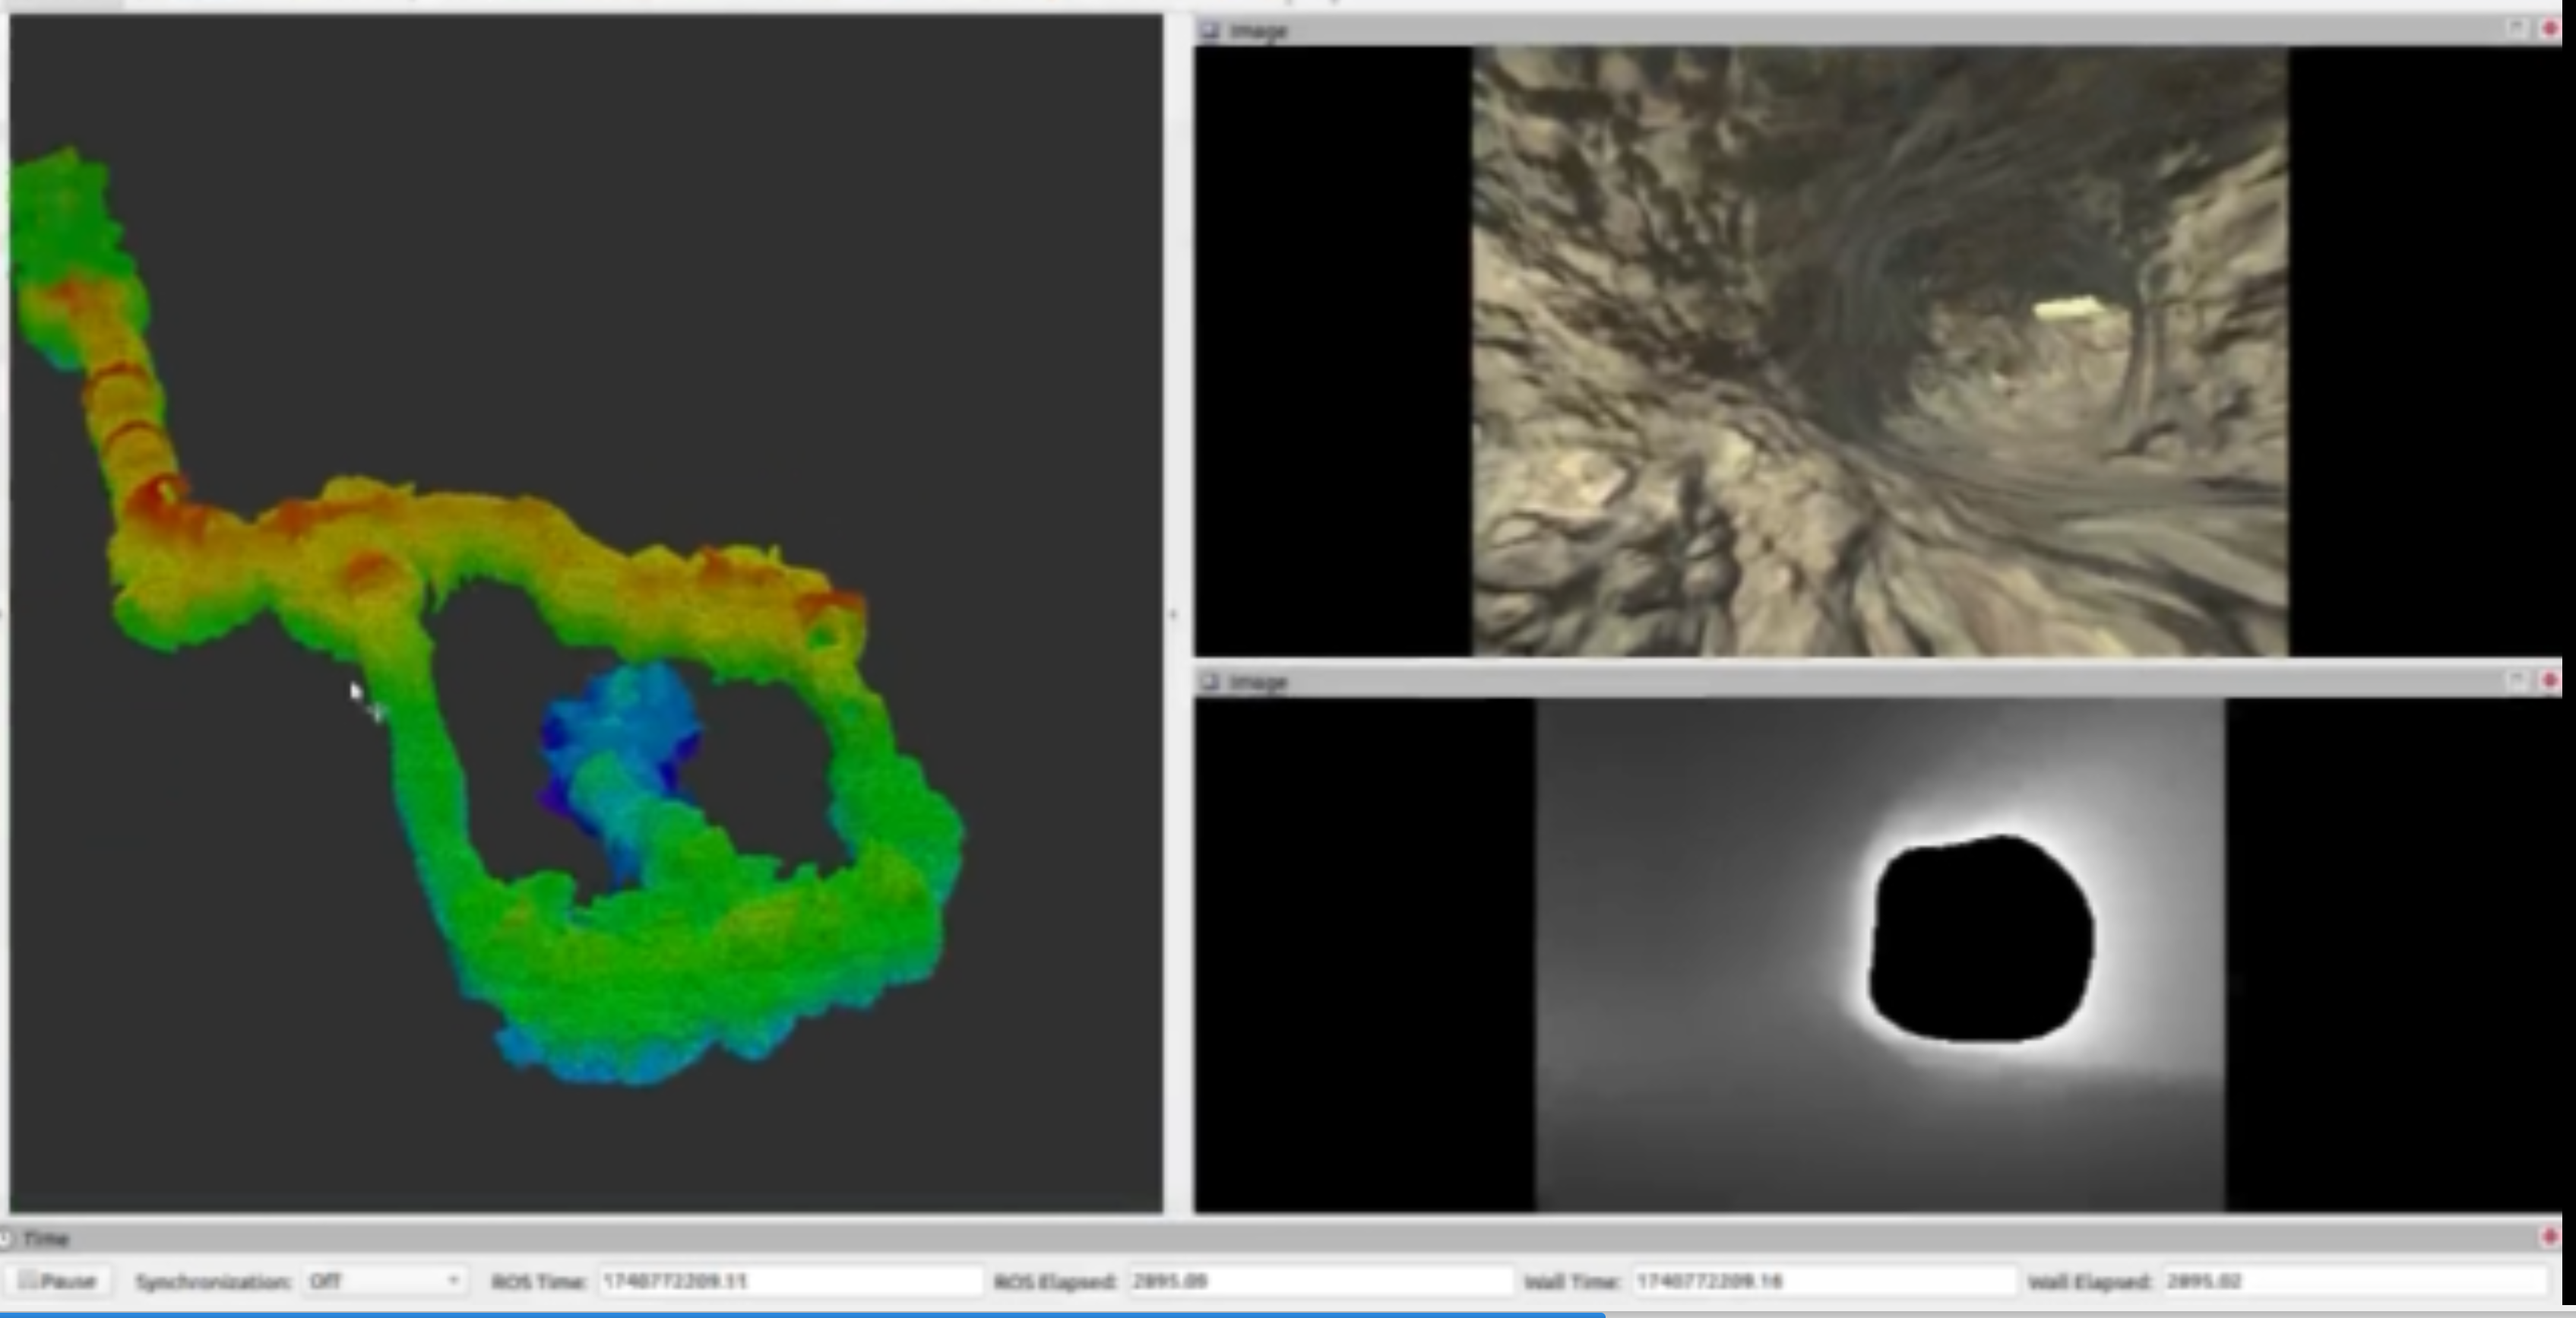
\includegraphics[width=0.5\textwidth]{assets/full_map}}
            \caption{A demo GUI showing the full map is detected and rendered}  
            \label{fig:GUI}
    \end{figure}

\section{Contributions}
\begin{outline}
    \1 Bingkun Huang: path planning, system integration.
    \1 Haowen Shi: UAV control module.
    \1 Siyan Li: trajectory generation, documentation.
    \1 Weili Tang: semantic camera, perception.
    \1 Zhenjiang Li: Octomap, build system, manual control.
\end{outline}





















\bibliographystyle{IEEEtran}
\bibliography{references}



\end{document}
